\documentclass[10pt,twocolumn,letterpaper]{article}

\usepackage{statcourse}
\usepackage{times}
\usepackage{epsfig}
\usepackage{graphicx}
\usepackage{amsmath}
\usepackage{amssymb}

% Include other packages here, before hyperref.

% If you comment hyperref and then uncomment it, you should delete
% egpaper.aux before re-running latex.  (Or just hit 'q' on the first latex
% run, let it finish, and you should be clear).
\usepackage[breaklinks=true,bookmarks=false]{hyperref}


\statcoursefinalcopy


\setcounter{page}{1}
\begin{document}


%%%%%%%%%%%%%%%%%%%%%%%%%%%%%%%%%%%%%%%%%%%%%%%%%%%%%%%%%%%%%%%
% DO NOT EDIT ANYTHING ABOVE THIS LINE
% EXCEPT IF YOU LIKE TO USE ADDITIONAL PACKAGES
%%%%%%%%%%%%%%%%%%%%%%%%%%%%%%%%%%%%%%%%%%%%%%%%%%%%%%%%%%%%%%%



%%%%%%%%% TITLE
\title{An Approach to Mammary Cancer Diagnosis Based on Mammography}

\author{First Author\\
{\tt\small zni32@wisc.edu}
\and
Second Author\\
{\tt\small secondauthor@wisc.edu}
\and
Third Author\\
{\tt\small thirdauthor@wisc.edu}
}

\maketitle
%\thispagestyle{empty}



% MAIN ARTICLE GOES BELOW
%%%%%%%%%%%%%%%%%%%%%%%%%%%%%%%%%%%%%%%%%%%%%%%%%%%%%%%%%%%%%%%


%%%%%%%%% ABSTRACT
\begin{abstract}
   The abstract for your project goes here. The length of the abstract
   should be between 200-250 words. Tips for writing a good abstract
   can be found at \url{https://writing.wisc.edu/Handbook/presentations_abstracts.html}.
\end{abstract}

%%%%%%%%% BODY TEXT
\section{Introduction}

In the America, about 1 in 8 women will develop breast cancer at some point in their lifetime. Over 40,000 women are expected to die in 2018 from this disease. Mammogram screens, which are X-Ray pictures of the breast, are currently the best test for doctors to identify this cancer as early as possible. Sometimes, they are able to identify the disease up to two years before it can be physically felt, which can be crucial in preventing fatality.

It’s important to note the difference between two types of mammograms: screening and diagnostic. Mammogram screens are routinely implemented to check for any abnormalities. If an abnormality is found, it calls for further inspection and possibly a follow up diagnostic test. This test could be a diagnostic mammogram or one of the several other alternatives, such as a biopsy. The diagnostic test will result in a benign or malignant decision for the tumor. This project is focuses on screening mammograms, which try to detect and classify any abnormalities that might signify cancer and lead to additional testing.  

Despite the benefits from mammogram screens, there are serious downfalls. For starters, nearly 1 in 5 screenings will not detect breast cancer if it is present, resulting in a false-negative.  Estimates suggest that approximately 10-20\% of mammograms without breast cancer will be incorrectly diagnosed with an abnormality, resulting in a false-positive as well. Nearly half of women who get an annual mammogram over a 10-year period will receive an incorrect positive test result because of this high false-positive rate.  Not only does this create inefficiencies in the healthcare system, but it also leads to emotional stress and anxiety in women who are incorrectly diagnosed with cancer. Because of these downfalls, many people have questioned whether mammograms should be routinely implemented. 

The previous reasons have lead to our motivation in this topic. More effective diagnosis could reduce over-diagnosis, over-treatment, fatality rates, healthcare costs, and financial and emotional burden put on patients. Even marginally small improvements could prove quite meaningful; over 33 million mammograms are performed each year in the United States. 

\section{Related Work}

Within the past five years, there’s been an increase in research focused on improving the various stages of mammograms via machine learning. From literature, most work falls under two categories: Multi-Stage and End-to-End approaches. The process from screening to diagnosis can be split into three stages: detection, further analysis, and final diagnosis. There has been some, but not much, research on End-to-End approaches, which attempt to tackle all three stages of mammogram assessment. 

\url{https://arxiv.org/pdf/1703.07047.pdf}

Most research, however, focuses on addressing a singular stage in this process, such as mass detection. Most similar to our project is the additional research that’s been done trying to classify specific regions of interest. Much of this research addresses classification by using deep convolutional neural networks, which is also the method we will applying. Some of the techniques employed are more advanced and beyond the scope of our knowledge. This research also varies on the resolution of the images used as well as the preprocessing techniques. 

High-Resolution Breast Cancer Screening with Multi-View Deep Convolutional Neural Networks (KJ Geras, et al). 

%{Table \ref{tab:some-table} shows an example for formatting a table.

\section{Proposed Method}

\subsection{kNN}

K-nearest neighbors algorithm (kNN) is a non-parametric method used for classification and regression. Here, we will use the kNN to solve the classification problem. In k-NN classification, the output is a class membership. An object is classified by a majority vote of its neighbors, with the object being assigned to the class most common among its k nearest neighbors (k is a positive integer, typically small). If k = 1, then the object is simply assigned to the class of that single nearest neighbor.

\begin{figure}[ht]
\begin{center}
   \includegraphics[width=0.8\linewidth]{figures/kNNalgorithm.png}
\end{center}
   \caption{Illustration of kNN for a 3-class problem with k=5.}
\label{kNNalgorithm}
\end{figure}

The K-Nearest Neighbor classifier usually applies either the Euclidean distance or the cosine similarity between the training samples and the test sample. And here we use the Euclidean distance. The Euclidean distance between a training sample and a test sample can be derived as follows:

Let $X_{i}$ be an input sample with $p$ features $(x_{i1}, x_{i2}, \ldots, x_{ip})$

Let n be the total number of input samples (i = 1, 2, …, n)

Let p be the total number of features (j = 1, 2, …, p)

The Euclidean distance between sample $X_{i}$ and $X_{t}(t = 1, 2, \ldots, n)$ can be defined as

$$d(x_{i},x_{t})=\sqrt{(x_{i1}-x_{t1})^2+(x_{i2}-x_{t2})^2+\ldots+(x_{in}-x_{tn})^2}$$

The nearest sample is determined by the closest distance to the test sample. The K-NN rule is to assign to a test sample the majority category label of its K-Nearest training sample.

In this project, if we apply the kNN directly to the mammographies, the sample is the matrix of mammographies, which can be treated as the following form.

$$<x_{1},x_{2},\ x_{3},\ \ldots,\ x_{n}>$$

where $x_{i}$ is 1024$\times$1 vector and n=1024.



\subsection{Random forests}

Random forests or random decision forests are an ensemble learning method for classification, regression and other tasks that operates by constructing a multitude of decision trees at training time and outputting the class that is the mode of the classes (classification) or mean prediction (regression) of the individual trees.\cite{ho1995random} \cite{barandiaran1998random} Compared with common decision, random forests can effectively correct for decision trees' habit of overfitting to their training set.

\paragraph{Bagging} The training algorithm for random forests applies the general technique of bootstrap aggregating, or bagging, to tree learners. Given a training set $X = x_1, \ldots, x_n$ with responses $Y = y_1, \ldots, y_n$, bagging repeatedly ($B$ times) selects a random sample with replacement of the training set and fits trees to these samples:\\

For $b = 1, \ldots, B$:

1.Sample, with replacement, $n$ training examples from $X, Y$; call these $X_b, Y_b$.

2.Train a classification or regression tree fb on $X_b, Y_b$.\\

After training, predictions for unseen samples $x'$ can be made by averaging the predictions from all the individual regression trees on $x'$:

$${\displaystyle {\hat {f}}={\frac {1}{B}}\sum _{b=1}^{B}f_{b}(x')}$$

or by taking the majority vote in the case of classification trees.

This bootstrapping procedure leads to better model performance because it decreases the variance of the model, without increasing the bias. This means that while the predictions of a single tree are highly sensitive to noise in its training set, the average of many trees is not, as long as the trees are not correlated. Simply training many trees on a single training set would give strongly correlated trees (or even the same tree many times, if the training algorithm is deterministic); bootstrap sampling is a way of de-correlating the trees by showing them different training sets.

Additionally, an estimate of the uncertainty of the prediction can be made as the standard deviation of the predictions from all the individual regression trees on x':

$${\displaystyle \sigma ={\sqrt {\frac {\sum _{b=1}^{B}(f_{b}(x')-{\hat {f}})^{2}}{B-1}}}.}$$

The number of samples/trees, $B$, is a free parameter. Typically, a few hundred to several thousand trees are used, depending on the size and nature of the training set. An optimal number of trees $B$ can be found using cross-validation, or by observing the out-of-bag error: the mean prediction error on each training sample $x_i$, using only the trees that did not have $x_i$ in their bootstrap sample. The training and test error tend to level off after some number of trees have been fit.

\paragraph{From bagging to random forests} The above procedure describes the original bagging algorithm for trees. Random forests differ in only one way from this general scheme: they use a modified tree learning algorithm that selects, at each candidate split in the learning process, a random subset of the features.

\url{https://en.wikipedia.org/wiki/Random_forest#cite_note-elemstatlearn-3}

\subsection{ANN}

An artificial neural network(ANN) is a network of simple elements called artificial neurons, which receive input, change their internal state (activation) according to that input, and produce output depending on the input and activation. ANN can be divided into a lot of classifications according to the structure of the model (The configurations of VGG models are showed in Figure \ref{VGG}). And what we used in the report is VGG16. VGG16 is a basic method with totally 16 layers in the model. \cite{simonyan2014very} 

\begin{figure}[t]
\begin{center}
   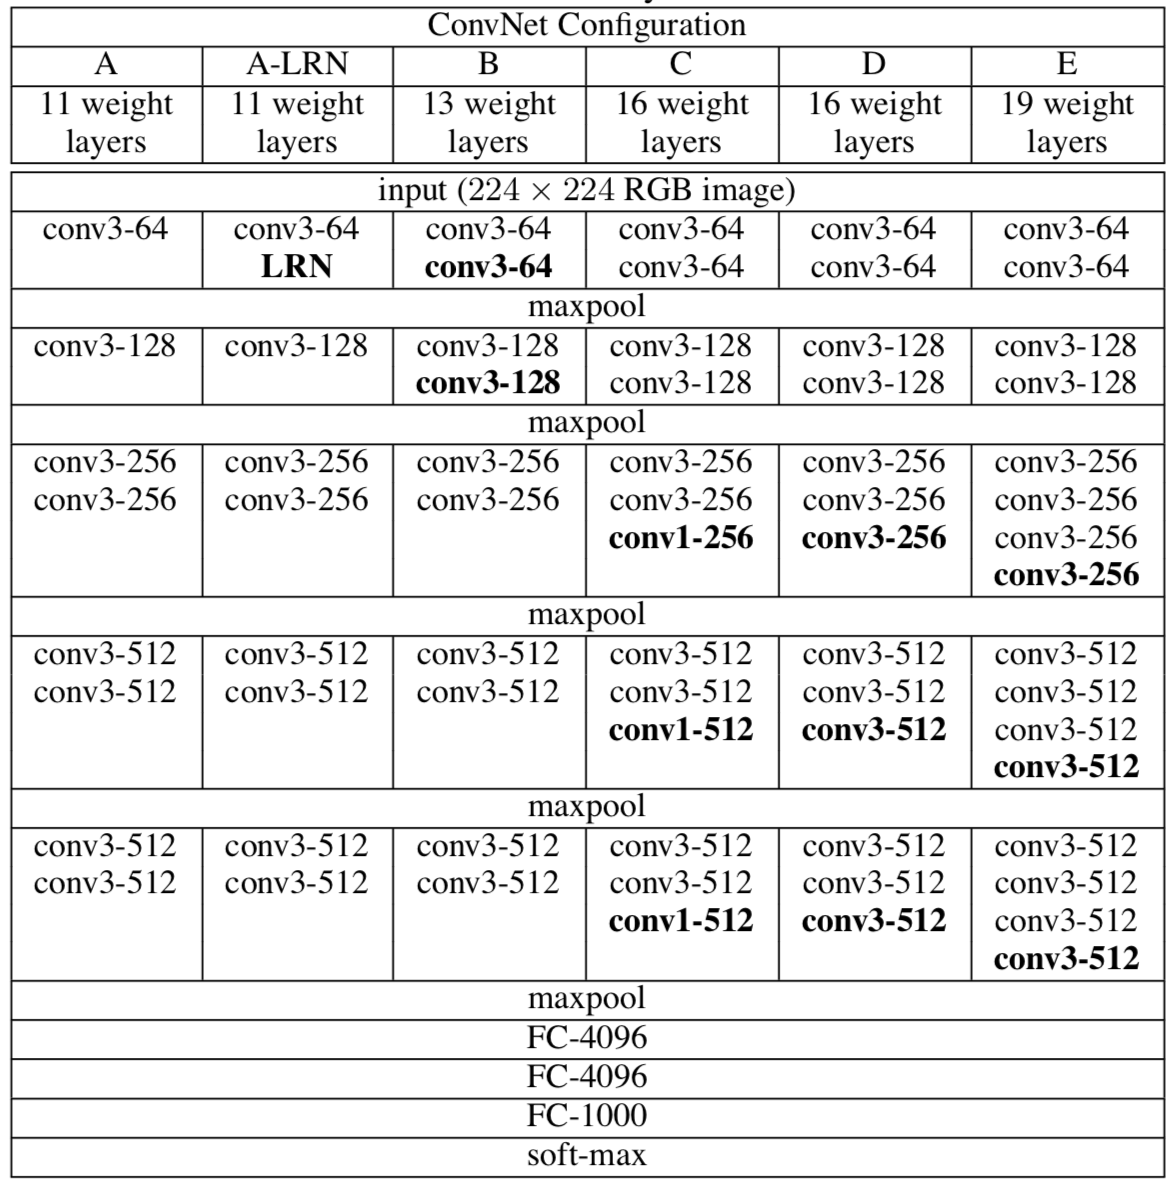
\includegraphics[width=1\linewidth]{figures/VGG.png}
\end{center}
   \caption{\textbf{ConvNet configurations} (shown in columns). The depth of the configurations increases from the left (A) to the right (E), as more layers are added (the added layers are shown in bold). The convolutional layer parameters are denoted as “conv⟨receptive field size⟩-⟨number of channels⟩”. The ReLU activation function is not shown for brevity.}
\label{VGG}
\end{figure}

\section{Experiments}

\subsection{Dataset}

The data set is the Mammographic Image Analysis Society (MIAS)(\url{https://www.kaggle.com/kmader/mias-mammography}) database provide by university of cambrige, which contains 322 images of mammography along with its conditions(see Figure \ref{datasample}).

\begin{figure}[h]
\begin{center}
   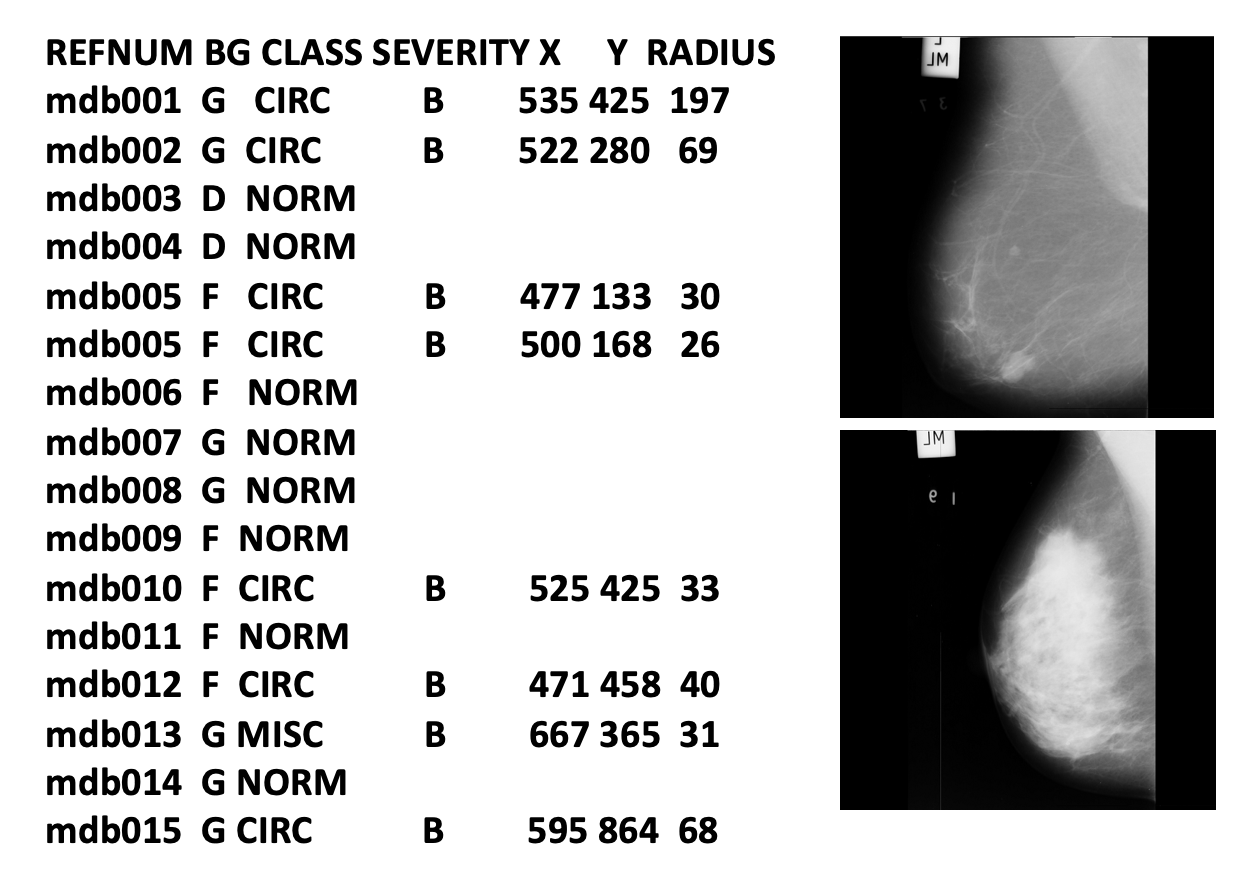
\includegraphics[width=1\linewidth]{figures/datasample.png}
\end{center}
   \caption{Samples of MIAS dataset.}
\label{datasample}
\end{figure}

 
The first column reference the number of the image. The second column is the character of background tissue: where F means Fatty, G means Fatty-glandular and D for Dense-glandular. 
The third column is quite important for it’s the label column of the class of abnormality present.

\subsection{Software}

Python

\subsection{Data preprocessing}

The data pre-processing is very important for complex data set. After checking the images of mammography, we noticed several problems. 

Firstly, the images are arranged in pairs, where each pair represents the left (even filename numbers) and right mammograms (odd filename numbers) of a single patient. So the first thing is to reverse some of the images to make all of them face the same side. 

Secondly, the images are recorded not so well. There are many bright spots and lines in the dark areas of images. We should dealing with these parts very carefully. Generally, we erase the noise on the right and left side of the breast shape by setting the pixels be zero. But images with id 287 and 280 are exceptions. So we designed special functions to pre-process these pictures.

\begin{figure}[t]
\begin{center}
   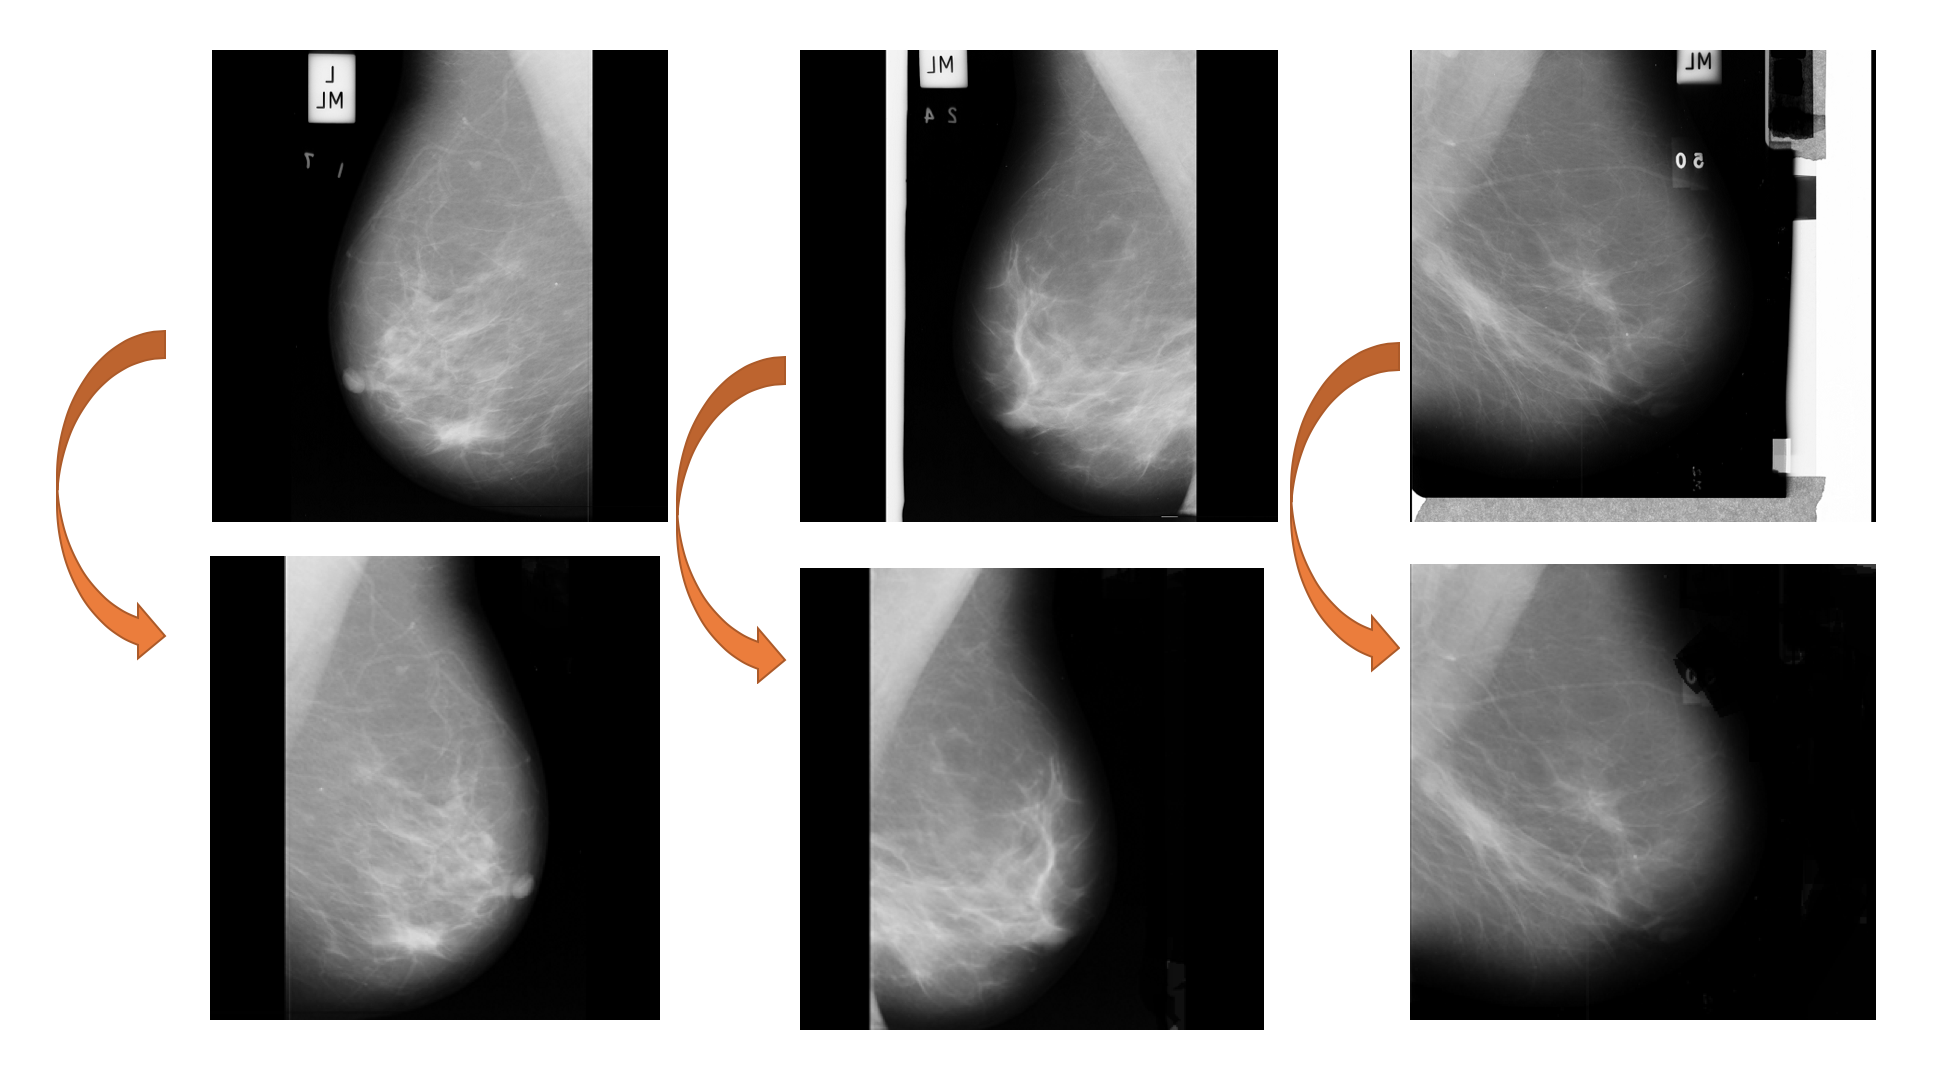
\includegraphics[width=1\linewidth]{figures/preprocessing.png}
\end{center}
   \caption{Three samples of preprocessing. (mirroring and noise removing)}
\label{preprocessing}
\end{figure}

Another problem is the high dimension. The images are in shape 1024*1024. This will cost us a lot of time to train the model. So we use the PCA method to deduct the dimension to 4*1024 which still save 97\% of the information, but only use 1/256 of the original features. 

\subsection{kNN and random forest}

kNN and random forests are two very basic but effective machine learning method. Using kNN and random forests is quite simple for the data has been processed well enough. We simply split the data set into training set(70\%) and test set(30\%). Since the amount of samples is very small, the number of a certain class may be only 7 or 8, after splitting the original data set into training set and test set, there is no more space to do cross validation.

We tried several coefficients for the two models. After several experiments we find that kNN and random forests both reach an accuracy of 60\% to 65\%. The accuracy reached the highest when n=9 for kNN, which is 64.65\%. While the highest accuracy for random forests is 63.64\% when n\_estimators = 20. It seems kNN has a higher accuracy than random forest, however, if we see it carefully, none of the abnormal class other than CALC is predicted correctly. So basically, it’s a predictor considering everything normal. As for random forest, though it has a lower accuracy, the recall scores show that this predictor successfully predict a few samples for different classes. I believe with a larger amount of samples, we will get a better performance. (see Figure \ref{kNN1} and Figure \ref{rf1})

\begin{figure}[h]
\begin{center}
   \includegraphics[width=1\linewidth]{figures/kNN1.png}
\end{center}
   \caption{The accuracy of raw kNN algorithm.}
\label{kNN1}
\end{figure}

\begin{figure}[h]
\begin{center}
   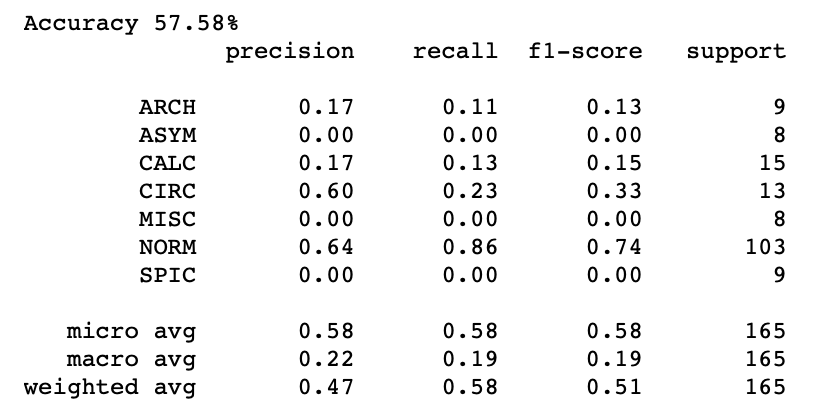
\includegraphics[width=1\linewidth]{figures/rf1.png}
\end{center}
   \caption{The accuracy of raw random forests algorithm.}
\label{rf1}
\end{figure}

It’s important to emphasize that the cases in this dataset is very complicated. It’s harder than the original image processing. The abnormality we are trying to find is located in different places in the images, the breast part locates in different places, and there is even some images with two different types of abnormality. So we need to do more work when we are using kNN and random forest. This will be introduced in the next part.

\subsection{Improved kNN and random forest}

From the previous result, we can see that the accuracy of the specific classification of the cancer type is extremely bad, which is even all zero (kNN) and about 40\% for random forest. We can see that it is not only the problem of the dataset, but also due to the basic structure of the algorithms. From the previous research, we can see that there are some featured problems causing the low accuracy, and in this part, we will try to do some targeted changes to improve the kNN and Random forests. Additionally, to get the more useful result, we reduce the labels into just Normal and Cancer. Then, the problem becomes a Binary classification problem. 

As we know from the previous parts, one kind of problems may occur when the position of the cancer core differs. While the whole image is rather big (1024x1024) and the radius of the cores are mostly about 40, the position of the cancer core in the picture has a very vital impact on the accuracy. Thus, we tried to split the whole pic into the small pieces, like small squares. We use the coordinates (x, y) provided in the labels and the median of the radius to extract the cores out of the picture. Then, we randomly pick up squares of the same size from the normal samples. Due to this operation, the effect of the position of cores can be erased because if the cores appear on the picture, they will take the majority of the area. Another benefit of this operation is that the size of the picture has been successfully reduced to 20x20, which is rather smaller than the raw samples. This means the computational efficiency has been improved a lot.

Another problem is the dataset itself. We can see that besides the distribution problem, the whole dataset only contains 330 samples, while some of them are still repetitive. Small size means the outliers may have a big impact on the final result, and also will easily lead to overfitting problems for the models. For the distribution problem, we tried replication way to balance the distribution. Here, for the data size problem, we considered some oversampling techniques. Using elastic distortions, one image can be used to generate many images that are real-world feasible and label preserving. There are several types of elastic distortions, like perspective transforms, rotation, shearing, cropping, and random erasing. With only a few operations, we can produce a large number of samples which is applicable in the model. Here, because the size of the samples is important in our classification, we decide to choose the size preserving ways, rotation and transition. To control the distribution of the dataset, we keep the ratio between the core parts and the normal parts 1:2. 

Because the size of the samples is already small enough, we didn’t use PCA method to reduce the dimension of the samples this time. We directly apply the kNN method to the samples. We split the whole samples into training set and test set. Then we use the kNN and random forests to see wether the outcome improved. From the code, we can see that the accuracy of kNN has been increased to 86.15\% and the accuracy of the random forests has been increased to the 84.62\% which is obviously better compared with former results. (see Figure \ref{kNN2} and Figure \ref{rf2})

\begin{figure}[h]
\begin{center}
   \includegraphics[width=1\linewidth]{figures/kNN2.png}
\end{center}
   \caption{The accuracy of improved kNN algorithm.}
\label{kNN2}
\end{figure}

\begin{figure}[h]
\begin{center}
   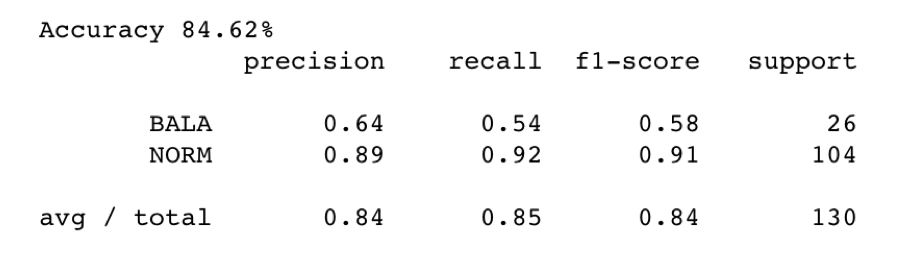
\includegraphics[width=1\linewidth]{figures/rf2.png}
\end{center}
   \caption{The accuracy of improved random forests algorithm.}
\label{rf2}
\end{figure}

However, the most important part is still a struggle place in this method. The accuracy of the classification of whole mammography is still very low. We tried to use the expectation of the number of negative squares to determine whether the sample is normal or abnormal. But the result is not adorable, which may due to the accuracy of the algorithm being still low. We are still finding how to make it a more applicable method.

\subsection{ANN}

Compared with kNN and random forest, ANN is much better to deal with this kind of problems. 

Convolutional Neural Network is really a good method to deal with images. We tried VGG16 in this project (the code and pre-trained model can be found in \url{https://www.kaggle.com/kmader/pretrained-vgg16-for-mammography-classification/notebook}). VGG16 is a basic method with totally 16 layers in the model. To use this method, we also balanced the distribution of the dataset since there are 70 percent of samples with class Normal. Then, from the result, we can see that compared with kNN and random forest, ANN is much outstanding. (See Figure \ref{ANN})

\begin{figure}[h]
\begin{center}
   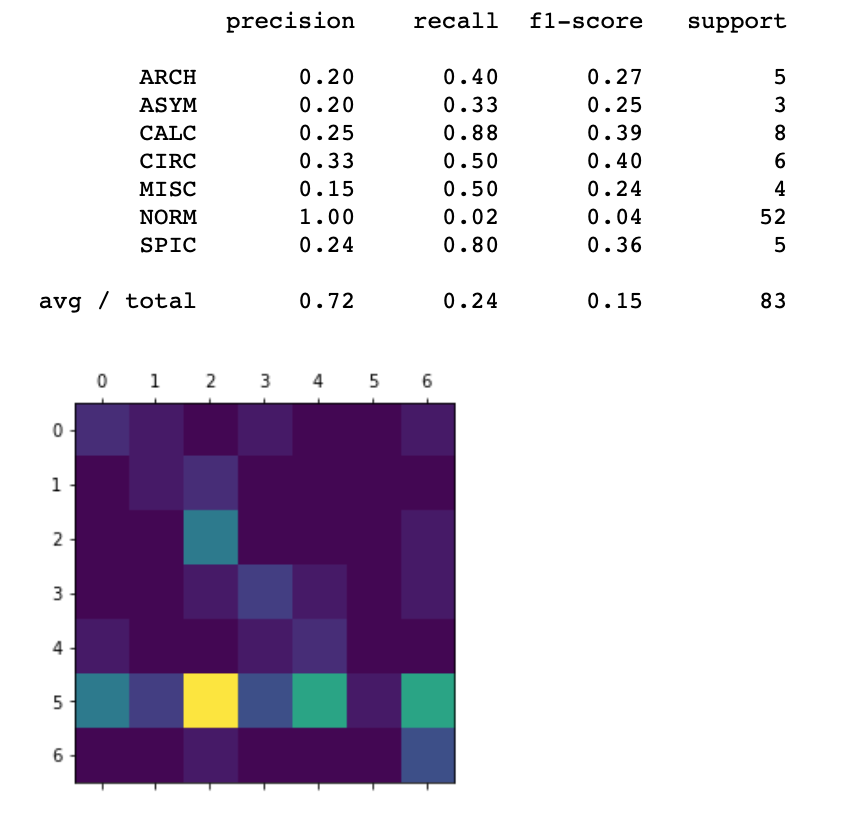
\includegraphics[width=1\linewidth]{figures/ANN.png}
\end{center}
   \caption{The accuracy of ANN VGG16.}
\label{ANN}
\end{figure}

\section{Results and Discussion}

From the result from the experiments (see Table \ref{result}), we can see that while treating well processed datasets, kNN and random forests are truly efficient and well-performed. However, when facing the dataset that is not that standard, their limitations are undoubtedly revealed. We can see that kNN and random forests are easily affected by the position and size of the cancer core. And the degree of the gray scale which is determined by the thickness of the fat and muscle also result in the misclassification in the model. Even though the improved kNN and random forest's results seem perfect, the most important part is still not solved in this report. That is the classification of the whole mammography. We are still work on this part to find a way to complish it.

Compared with the kNN and random forest, ANN is much more robust to deal with the noised dataset. While treating the 7 classification problem, we can see that ANN's precision of the classification is much more acceptable than kNN, which is average 72\% and its recall ratios for abnormal classes are all high enough. However, it is much more time-consuming than the other two in this problem, while it will use about 380s every epoch and about half an hour all 5 epochs (differs on different computers). Besides, from the outcome of ANN in this problem, we can see that the recall ratio of normal samples are really low. That is because the ANN algorithm class almost all the samples into abnormal ones. This may caused by the distribution balance part. But due to the time limitation, we can't find out why. We will try to fix this problem in the future study.

\begin{table}[h]
\begin{center}
\begin{tabular}{|l|c|c|}
\hline
Method & Precision & Recall\\
\hline\hline
kNN & $39 \pm 3$ \% & $61 \pm 3$ \%\\
R. F. & $47 \pm 3$ \% & $58 \pm 3$ \%\\
kNN (Binary) & $85 \pm 3$ \% & $86 \pm 3$ \%\\
R. F. (Binary) & $84 \pm 3$ \% & $85 \pm 3$ \%\\
ANN & $72 \pm 3$ \% & $24 \pm 3$ \%\\
\hline
\end{tabular}
\end{center}
\label{result}
\caption{The accuracy of the all five experiments.}
\end{table}

\section{Conclusions}

\section{Acknowledgements}

\section{Contributions}

\textbf{Project Report (writing)}

Introduction - Dan

Related Work - Dan

Proposed Method - Nemo, Zheng Ni

Experiments - Nemo, Zheng Ni

Results and Discussion - Dan, Zheng Ni

Conclusions - Dan

Contributions - Dan, Zheng Ni, Chong Wei\\

\textbf{Computational Tasks}

Preprocessing - Nemo, Zheng Ni

Model Selection- Zheng Ni 

Evaluation and Parameter Tuning - Nemo, Zheng Ni

Result evaluating - Nemo, Dan

{\small
\bibliographystyle{ieee}
\bibliography{ref}
}

\end{document}
